\documentclass[14pt]{article}

\usepackage[utf8x]{inputenc}
\usepackage[russian]{babel}
\usepackage{graphicx}
\graphicspath{{images/}}
\DeclareGraphicsExtensions{.pdf,.png,.jpg}

\usepackage{amsmath}
\usepackage{pgfplots}

\usepackage{geometry} % Меняем поля страницы
\geometry{left=2cm}% левое поле
\geometry{right=1.5cm}% правое поле
\geometry{top=2cm}% верхнее поле
\geometry{bottom=2cm}% нижнее поле

\renewcommand{\theenumi}{\arabic{enumi}}
\renewcommand{\labelenumi}{\arabic{enumi}}
\renewcommand{\theenumii}{.\arabic{enumii}}
\renewcommand{\labelenumii}{\arabic{enumi}.\arabic{enumii}.}
\renewcommand{\theenumiii}{.\arabic{enumiii}}
\renewcommand{\labelenumiii}{\arabic{enumi}.\arabic{enumii}.\arabic{enumiii}.}

\begin{document}
\begin{titlepage}
	\begin{center}
		\fontsize{18pt}{20pt}\selectfont
		\textbf{Работа 3.2.6.}	
	
		\vspace{5cm}
		\fontsize{24pt}{25pt}\selectfont
		Баллистический гальванометр
	\end{center}
	\begin{flushright}
		\fontsize{18pt}{20pt}\selectfont
		\vspace{14cm}
		\hspace{-3cm}
		\textit{Корнеев Е.С.}
	\end{flushright}		
\end{titlepage}

\begin{center}
	\fontsize{16pt}{18pt}\selectfont	
	Баллистический гальванометр
\end{center}


\fontsize{14pt}{16pt}\selectfont
\vspace{1cm}
\textbf{Цель работы:} изучение работы высокочувствительного зеркального гальванометра магнитоэлектрической системы в режимах измерения постоянного тока и электрического заряда.

\vspace{0.5cm}
\textbf{Оборудование:} зеркальный гальванометр с осветителем и шкалой, источник постоянного напряжения, делитель напряжения, магазин сопротивлений, эталонный конденсатор, вольтметр, переключатель, ключи, линейка. 

\vspace{1cm}
Баллистический гальванометр - электроизмерительный прибор магнитоэлектрической системы, отличающийся высокой чувствительностью к току и обладающий сравнительно большим периодом колебаний рамки. 

Главной частью баллистического гальванометра является подвешенная на вертикальной нити рамка, помещённая в поле постоянного магнита. Вырез цилиндрической формы в полюсах магнита и ферромагнитный цилиндр на оси системы делают поле в зазоре радиальным (рис. 1). Скреплённое с рамкой зеркальце служит для измерения угла поворота рамки. К рамке прикреплён полый цилиндр, который сильно увеличивает момент инерции и, следовательно, период колебаний подвижной системы, не очень её утяжеляя. Магнит и подвижная система заключены в защитный кожух. В баллистических гальванометрах применяют сильные постоянные магниты и рамки с большим количеством витков, подвешенные на тонких нитях с малой упругостью.

Баллистический гальванометр позволяет измерять как постоянный ток (стационарный режим), так и заряд, протекший через рамку за некоторое время (баллистический режим). В баллистическом режиме гальванометр может работать, если время протекания заряда много меньше периода собственных колебаний подвижной рамки. Поэтому период колебаний рамки делают большим (5+ 15 с). Это время учитывает реакцию экспериментатора, которому надо успеть сделать отсчёт максимального отклонения рамки.

\textbf{Уравнение движения подвижной системы.} На помещенную в магнитное поле обтекаемую током рамку гальванометра действуют следующие моменты сил: момент закрученной нити, момент магнитных сил и тормозящий момент, зависящий от сил сопротивления воздуха и от вихревых токов, вызывающих электромагнитное торможение. Рассмотрим каждый из этих моментов в отдельности.

Механический момент $M_1$ упругих сил нити пропорционален углу поворота рамки
\begin{equation}
	M_1 = -D\varphi
\end{equation}
где $D$ - модуль кручения нити, а $\varphi$ - угол поворота рамки от положения равновесия.

Если рамка с числом витков $N$, обтекаемая током $I$, помещена в магнитное поле с индукцией $B$, то на боковые стороны рамки (перпендикулярные чертежу на рис. 1) действуют силы, равные $lNBI$, где $l$ - длина боковой стороны. Обозначив через $r$ расстояние от боковой стороны до оси вращения, найдём момент пары сил 
\begin{equation}
	M_2 = 2rlBNI = BSNI
\end{equation}
где $S$ - площадь одного витка рамки.

\begin{figure}[h!]
	\center{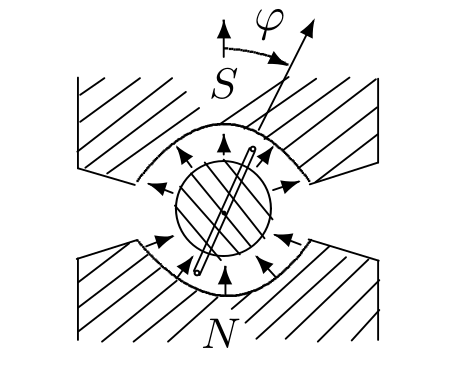
\includegraphics[width = 6cm]{1}}
	\caption{Рамка с током в магнитном поле}
	\label{fig:image}
\end{figure}

Тормозящий момент складывается из моментов сил электромагнитного торможения и сил трения о воздух. В рамке, движущейся в магнитном поле с угловой скоростью $\dot{\varphi}$, наводится ЭДС индукции:
$$
	\varepsilon_{\text{инд}} = -\frac{d\Phi}{dt} = -BSN\dot{\varphi}
$$
где $\Phi$ - магнитный поток, пронизывающий рамку. Пренебрегая самоиндукцией рамки, можно считать, что эта ЭДС вызывает ток индукции 
$I_{\text{инд}} = -BNS\dot{\varphi}/R_{\Sigma}$. Здесь $B$ - полное сопротивление цепи, состоящее из сопротивления рамки $R_0$ и сопротивления внешнего участка цепи $R$:
$R_\Sigma = R_0 + R$. Тормозящий момент
\begin{equation}
	M_3 = BNSI_{\text{инд}} = -\frac{(BNS)^2}{R_\Sigma}\dot{\varphi}
\end{equation}

Обычно этот момент значительно превосходит момент сил трения рамки о воздух, которым мы и пренебрежём для простоты расчёта.

Уравнение движения рамки имеет вид
$$
	J\ddot{\varphi} = \Sigma M
$$

где $j$ - момент инерции подвижной системы, а $\Sigma M$ - сумма моментов всех сил, действующих на рамку; подставляя (1), (2) и (3), получим
$$
	J\ddot{\varphi} + \frac{(BSN)^2}{R_\Sigma}\dot{\varphi} + D\varphi = BSNI
$$

Разделим обе части уравнения на $J$ и введём обозначения
\begin{equation}
	\frac{(BSN)^2}{JR_\Sigma} = 2\gamma,~~~\frac{D}{J} = \omega_0^2,~~~\frac{BSN}{J} = K
\end{equation}

Уравнение движения рамки примет вид
\begin{equation}
	\ddot{\varphi} + 2\gamma\dot{\varphi} + \omega_0^2\varphi = KI
\end{equation}

Величина $\gamma$ называется \textsl{коэффициентом затухания} подвижной системы гальванометра, $\omega_0$ - \textsl{собственной частотой} колебаний рамки.

Следует отметить, что ток $I$ в уравнении (5) определяется величиной ЭДС $\varepsilon$ внешнего источника, к которому подключён гальванометр: $I = \varepsilon/R_\Sigma$, а влияние индукционного тока, тормозящего движение рамки, отражает слагаемое, пропорциональное $\dot{\varphi}$.

\textbf{Режим измерения постоянного тока.} Если через рамку пропускать постоянный ток (достаточно долго, чтобы затухли колебания подвижной системы), то в уравнении (5) можно положить $\ddot{\varphi} = \dot{\varphi} = 0$, и угол поворота определится формулой
$$
	\varphi = \frac{K}{\omega_0^2}I = \frac{BSN}{D}I = \frac{I}{C_1}.
$$

Величина $C_1$ называется динамической постоянной гальванометра:
$$
	C_1 = \frac{I}{\varphi} = \frac{D}{BSN}
$$

\textbf{Свободные колебания рамки.} Исследуем свободное движение рамки (т. е. движение в отсутствие внешних источников тока, когда $I = О$).
Предположим, что выполнены следующие начальные условия:
\begin{equation}
	t = 0:~~~\varphi = 0,~~~\dot{\varphi} = \dot{\varphi_0}
\end{equation}

При этом уравнение (5) примет вид
\begin{equation}
	\ddot{\varphi} + 2\gamma\dot{\varphi} + \omega_0^2\varphi = 0
\end{equation}

Общее решение уравнения (7) имеет вид
\begin{equation}
	\varphi = A_1e^{\lambda_1t} + A_2e^{\lambda_2t}
\end{equation}
где $A_1$ и $A_2$ нужно выбрать так, чтобы удовлетворить начальным условиям. Здесь возможны следующие случаи:

1. $\gamma < \omega_0$ (колебательный режим).
Решение уравнения (7), удовлетворяющее начальным условиям (6), имеет в этом случае вид
\begin{equation}
	\varphi = \frac{\dot{\varphi_0}}{\omega}e^{-\gamma t}\sin(\omega t)
\end{equation}

где
\begin{equation}
	\omega^2 = \omega_0^2 - \gamma^2
\end{equation}

Движение рамки имеет колебательный характер и затухает со временем. Период колебаний равен
\begin{equation}
	T = \frac{2\pi}{\omega} = \frac{2\pi}{\sqrt{\omega_0^2 - \gamma^2}} = \frac{2\pi}{\sqrt{\frac{D}{J} - \frac{(BSN)^4}{(2JR_\Sigma)^2}}}
\end{equation}

Если затухание мало, $\gamma \ll \omega_0 (\omega \approx \omega_0)$, то движение рамки близко к синусоидальному:
\begin{equation}
	\varphi = \frac{\dot{\varphi_0}}{\omega_0}\sin(\omega_0t)
\end{equation}

2. $\gamma = \omega_0$ (критический режим). Решение уравнения (7) в этом случае имеет вид
\begin{equation}
	\varphi = \dot{\varphi_0}te^{-\gamma t}
\end{equation}

Движение не имеет колебательного характера: отклонённая подвижная система после отброса почти экспоненциально приближается к нулю.

З. Затухание велико, $\gamma > \omega_0$ (случай переуспокоенного гальванометра). Решение (7) в этом случае имеет вид
\begin{equation}
	\varphi = \frac{\dot{\varphi_0}}{\kappa}e^{\gamma t}\sh(\kappa t)
\end{equation}
где 
$$
	\kappa^2 = \gamma^2 - \omega_0^2
$$

Движение остаётся апериодическим, однако подвижная система приближается к равновесию медленнее, чем в критическом режиме. Режим измерения заряда. Как уже было отмечено, период свободных колебаний баллистического гальванометра благодаря искусственному увеличению момента инерции рамки оказывается очень большим (порядка десяти секунд). Если пропустить через рамку короткий импульс тока, то можно считать, что весь ток успевает пройти при неотклонённом положении рамки. Рамка, Однако, при этом получает толчок, в результате которого возникает движение, описываемое уравнением свободных колебаний (7) при начальных условиях (6).

Для вычисления скорости $\dot{\varphi_0}$, полученной в результате толчка, умножим уравнение (5) На $dt$ и проинтегрируем его по времени от О до $\tau$ - момента окончания токового импульса:
\begin{equation}
	\int_0^\tau \ddot{\varphi}dt + 2\gamma\int_0^\tau \dot{\varphi}dt + \omega_0^2\int_0^\tau \varphi dt = K \int_0^\tau Idt
\end{equation}

Рассмотрим первое слагаемое этого равенства:
\begin{equation}
	\int_0^\tau \ddot{\varphi}dt = \dot{\varphi}\big|_0^\tau = \dot{\varphi}(t)
\end{equation}

Второе и третье слагаемые пренебрежимо малы, поскольку, согласно принятому условию, к моменту времени $\tau$ рамка практически не сдвигается из положения равновесия.
\begin{equation}
	2\gamma\int_0^\tau \dot{\varphi}dt = 0,~~~\omega_0^2\int_0^\tau \varphi dt = 0
\end{equation}

где $q$ - полный электрический заряд, прошедший через рамку за время импульса. Строго говоря, заряд $q$ определяется не только током $I$, вызванным внешней ЭДС 
$\varepsilon$, но и током индукции, возникающим при движении рамки, но в наших условиях, согласно (17), вкладом индукционного тока можно пренебречь.

Итак, уравнение (15) сводится к следующему:
\begin{equation}
	\dot{\varphi}(t) = Kq
\end{equation}

Таким образом, при пропускании коротких импульсов тока через баллистический гальванометр начальная скорость движения рамки пропорциональна полному электрическому заряду, прошедшему через рамку за всё время импульса. Подставляя выражение (18) в решения (9), (13) или (14), легко увидеть, что наибольший угол, на который отклоняется рамка, также пропорционален $q$.

Величина $C_Q = q/\varphi_{max}$ называется баллистической постоянной гальванометра. Баллистическая постоянная наряду с динамической является важнейшей характеристикой гальванометра, но в отличие от динамической она существенно зависит от режима работы гальванометра (от сопротивления цепи).

Выбирая оптимальный режим работы, приходится одновременно исходить из двух противоречивых требований: желания получить максимальную чувствительность гальванометра к заряду и стремления по возможности сократить время, затрачиваемое на измерения.

Расчёт показывает, что максимальный отброс достигается при полном отсутствии затухания (тормозяший индукционный ток отсутствует
при обрыве в цепи):
\begin{equation}
	\varphi_{max~\text{св}} = \frac{\dot{\varphi}(t)}{\omega_0} = \frac{Kq}{\omega_0}
\end{equation}

В этом случае, однако, возникшие в результате отброса колебания рамки не будут успокаиваться, и прибор не скоро сможет быть использован для повторных измерений. Поэтому обычно заботятся о том, чтобы затухание гальванометра не было слишком малым. Кроме того, отметим, что затухание приводит к тому, что зайчик начинает вести себя более
спокойно и слабее реагирует на на посторонние электрические и механические импульсы.

Обычно удобнее всего работать в режиме, близком к критическому. При этом обеспечивается быстрое затухание колебаний, и чувствительность прибора достаточно велика.

Как следует из уравнения (13), в случае критического затухания
\begin{equation}
	\varphi_{max~\text{кр}} = \frac{Kq}{\omega_0e}
\end{equation}

Таким образом, в критическом режиме максимальное отклонение зайчика в $e$ раз меньше, чем в режиме свободных колебаний. Отсюда, в частности, следует, что отношение баллистических постоянных 
$$
	\frac{C_{Q_\text{кр}}}{C_{Q_\text{св}}} = e
$$

\vspace{1cm}
\textbf{А. Определение динамической постоянной}

\textbf{Экспериментальная установка.} Схема для исследования гальванометра в стационарном режиме представлена на рис. 2. Постоянное напряжение $U \approx 1.5$В снимается с блока питания и измеряется вольтметром $V$. Ключ $K_3$ позволяет менять направление тока через гальванометр $\text{Г}$, делитель напряжения - менять величину тока в широких пределах. Ключ $K_2$ служит для включения гальванометра, кнопка $K_1$ - для его успокоения. Магазин сопротивлений $R$ позволяет менять режим работы гальванометра от колебательного до апериодического.

\begin{figure}[h!]
	\center{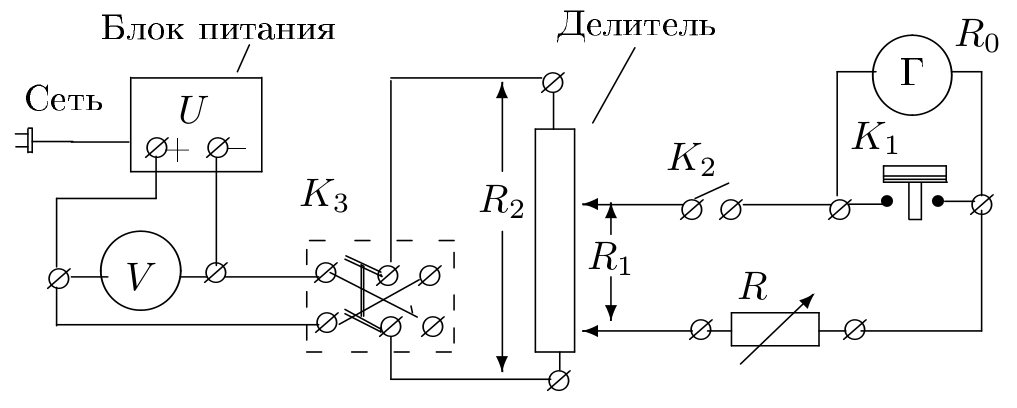
\includegraphics[width = 14cm]{2}}
	\caption{Схема установки для работы гальванометра в стационарном режиме}
	\label{fig:image}
\end{figure}

При малых $R_1$ сила тока, протекающего через гальванометр может быть вычислена по очевидной формуле:
\begin{equation}
	I = U_0\frac{R_1}{R_2}\frac{1}{R + R_0}
\end{equation}

где $U_0$ - показания вольтметра, $R_1/R_2$ - положение делителя, $R$ - сопротивление магазина, $R_0$ - внутреннее сопротивление гальванометра.

Угол отклонения рамки от положения равновесия измеряется с помощью осветителя, зеркальца, укреплённого на рамке, и шкалы, на которую отбрасывается луч света от зеркальца. Координата $x$ светового пятна на шкале связана с углом отклонения рамки формулой

$$
	x = a\tg(2\varphi)
$$

где $a$ - расстояние от шкалы до зеркальца. При малых углах можно считать, что $\varphi = x/2a$. Динамическую постоянную
\begin{equation}
	C_I = \frac{I}{\varphi} = \frac{2aI}{x}
\end{equation}

как правило, выражают в единицах $\left[\frac{A}{\text{мм}/\text{м}}\right]$ (ток $I$ измеряется в амперах, $x$ - в мм, $a$ - в метрах).

\vspace{1cm}
\textbf{Б. Определение критического сопротивления гальванометра}

Измерение критического сопротивления гальванометра можно выполнить с помошью той же цепи (рис. 2).

При больших $R$ свободное движение рамки имеет колебательный характер. С уменьшением $R$ затухание увеличивается (см. (4)), и колебательный режим переходит в апериодический.

Скорость затухания колебаний принято характеризовать \textsl{декрементом затухания} $\Delta$, равным отношению углов двух последовательных отклонений в одну сторону. С помощью (9) находим
$$
	\Delta = \frac{\varphi_n}{\varphi_{n+1}} = \frac{x_n}{x_{n+1}} = e^{\gamma T}
$$
где $T$ - период колебаний:
\begin{equation}
	T = \frac{2\pi}{\omega}
\end{equation}

Вместо декремента затухания $\Delta$ можно рассматривать \textsl{логарифмический декремент затухания} $\Theta$
\begin{equation}
	\Theta = \ln\Delta = \gamma T = \ln\frac{x_n}{x_{n+1}}
\end{equation}

Измеряя зависимость логарифмического декремента затухания от сопротивления внешней цепи, можно найти $R_{\text{кр}}$, т.е. значение $R$, при котором 
$\Theta \rightarrow \infty$. Измерения логарифмического декремента при сильном затухании затруднены, позтому исследуем зависимость $\Theta$ от $R$.
Подставляя в (24) значения Т из (23), $\omega$ из (10), $\gamma$ и $\omega_0$ из (4), получим
\begin{equation}
	\Theta = \gamma T = 2\pi\frac{\gamma}{\omega} = \frac{2\pi\gamma}{\sqrt{\omega_0^2 - \gamma^2}} = \frac{2\pi R_3}{\sqrt{(R_0 + R)^2 - R_3^2}},
\end{equation}

где введено обозначение
\begin{equation}
	R_3 = \frac{(BSN)^2}{2\sqrt{JD}} = R_0 + R_{\text{кр}}
\end{equation}

После простого преобразования равенства (25) получим
\begin{equation}
	\frac{1}{\Theta^2} = \frac{(R_0 + R)^2}{4\pi^2R_3^2} - \frac{1}{4\pi^2}
\end{equation}

Последнее уравнение, представленное на графике в координатах $X = (R_0 + R)^2$, $Y = 1/\Theta^2$, имеет вид прямой, угол наклона которой позволяет рассчитать критическое сопротивление:
\begin{equation}
	R_\text{кр} = \frac{1}{2\pi}\sqrt{\frac{\Delta X}{\Delta Y}} - R_0
\end{equation}

\vspace{1cm}
\textbf{В. Определение баллистической постоянной и критического сопротивления гальваномера, работающего в баллистическом режиме}

Для изучения работы гальванометра в режиме измерения заряда используется схема, представленная на рис. 3.

Система ключей устроена так, что нормально ключ $K_2$ замкнут, а ключи $K_3$ и $K_4$ разомкнуты. При нажатии на кнопку $K_0$ сначала размыкается ключ $K_2$, затем замыкается $K_3$ и через некоторое время - $K_4$.

При нормальном положении кнопки $K_0$ конденсатор $C$ заряжается до напряжения
$$
	U_C = \frac{R_1}{R_2}U_0
$$

\begin{figure}[h!]
	\center{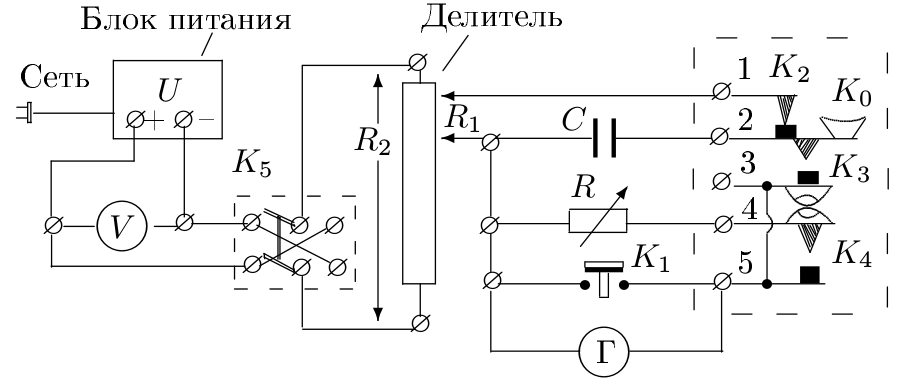
\includegraphics[width = 14cm]{3}}
	\caption{Схема установки для определения баллистической постоянной}
	\label{fig:image}
\end{figure}

Заряд конденсатора равен
\begin{equation}
	q = CU_C = \frac{R_1}{R_2}U_0C
\end{equation}

При нажатии на ключ $K_0$ конденсатор отключается от источника постоянного напряжения (размыкается ключ $K_2$) и подключается к гальванометру (замыкается ключ $K_3$).

Емкость конденсатора выбрана так, что к моменту замыкания ключа $K_4$ весь заряд успевает пройти через гальванометр, и рамка получает начальную скорость 
$\dot{\varphi}(\tau)$ (см. (18)). При этом можно считать, что отклонение рамки, происходящее за время, протекающее между замыканием ключей $K_3$ и $K_4$, равно нулю.

При замыкании ключа $K_4$ гальванометр шунтируется внешним сопротивлением $R$, и, в зависимости от величины этого сопротивления, движение рамки описывается одним из уравнений (12), (13) или (14).

Первый отброс зайчика $l_{max}$ после нажатия на кнопку $K_0$ зависит от сопротивления внешней цепи, подключенной к гальванометру. Для определения $R_{\text{кр}}$ используется то обстоятельство, что в критическом режиме максимальное отклонение зайчика в $e$ раз меньше, чем у гальванометра без затухания (см. (19) и (20)).

Следует помнить, что наблюдать колебания рамки при полном отсутствии затухания, конечно, невозможно, так как даже при разомкнутой внешней цепи ($R = \infty$) остаётся трение в подвеске и трение рамки о воздух. Величину максимального отклонения гальванометра без затухания $\varphi_0$ можно, однако, рассчитать, если при разомкнутой цепи измерены максимальное отклонение рамки $\varphi_1$ и логарифмический декремент затухания $\Theta_0$.

Из уравнений (9) и (24) следует, что при $\gamma \ll \omega_0$
\begin{equation}
	\varphi_0 = \varphi_1\cdot e^{\Theta_0/4}
\end{equation}

Баллистическая постоянная гальванометра $C_{Q_{\text{кр}}}$ $\left[\frac{\text{Кл}}{\text{мм}/\text{м}}\right]$ определяется
при критическом сопротивлении ($R = R_{\text{кр}}$):
\begin{equation}
	C_{Q\text{кр}} = \frac{q}{\varphi_{max~\text{кр}}} = 2a\frac{R_1}{R_2}\frac{U_0C}{l_{max~\text{кр}}}
\end{equation}

где $l_{max~\text{кр}}$ - величина первого отброса в критическом режиме, выраженная в делениях шкалы (мм), $a$ - расстояние от зеркальца до шкалы, выраженное в метрах, произведение $U_0C$ - заряд, выраженный в кулонах.

\newpage
\textbf{Ход работы}

1. Выставим делитель напряжения в отношении $R_1/R_2 = 1/2000$ и подберем $R$ такое, что зайчик будет отклоняться практически на всю шкалу. Такому $R$ соответствует значение 9 кОм. Также определим напряжение $U_0$: $U_0 = 65$ дел, причем мы измеряли в режиме 3В/150дел, откуда $U_0 = 1.3$В. При этом стоит отметить, что изначально зайчик был отклонен от нуля на 7мм, и эту величину вычтем из полученных значений, чтобы получить истинные значения отклонений. Также сразу отметим: $a = 1.1$м.

\begin{center}
\begin{tabular}{|c|c|c|c|c|c|c|c|}
\hline
$R$, кОм&$x$, см&$x_{real}$, см&$I$, нА\\
\hline
9&22,5&21,8&68\\
\hline
10&20,5&19,8&62\\
\hline
15&14,3&13,6&42\\
\hline
20&11,0&10,3&32\\
\hline
25&9,1&8,4&25\\
\hline
30&7,7&7,0&21\\
\hline
35&6,8&6,1&18\\
\hline
40&6,1&5,4&16\\
\hline
45&5,6&4,9&14\\
\hline
50&5,0&4,3&13\\
\hline
\end{tabular}
\end{center}

Примем погрешность $x_{real}$ равной 0.5см, так как снять точное значение довольно сложно в связи с нечеткостью изображения, а также потому что при определении этого значения мы вычитали небольшое начальное смещение, величина которого тоже определена с тоностью, не превосходящей цену деления линейки 1мм. На фоне этой погрешности мы можем пренебречь погрешностью $I$, учитывая, что погрешности величин, которые мы использовали при определении $I$, суммарно не превосходят 1\%. Таким образом, получим следующую зависимость $I(x)$:

\vspace{0.5cm}
\begin{tikzpicture}
\begin{axis}[
	height = 10cm,
	width  = 15cm,
	every axis y label/.style={at = {(ticklabel cs: 0.5)}, rotate = 90, anchor = near ticklabel},
	xlabel = {$x_{real}$, см},
	ylabel = {$I$, нА},
	grid   = major
]
\addplot+[
	only marks,
	error bars/.cd, 
	y dir = both, y explicit,
	x dir = both, x explicit,
	]
coordinates{
	(21.8, 68)	+-	(0.5, 0)
	(19.8, 62)	+-	(0.5, 0)
	(13.6, 42)	+-	(0.5, 0)
	(10.3, 32)	+-	(0.5, 0)
	(8.4, 25)	+-	(0.5, 0)
	(7.0, 21)	+-	(0.5, 0)
	(6.1, 18)	+-	(0.5, 0)
	(5.4, 16)	+-	(0.5, 0)
	(4.9, 14)	+-	(0.5, 0)
	(4.3, 13)	+-	(0.5, 0)
};

\addplot [mark = none]
coordinates{
	(21.8, 68.1617)
	(4.3, 12.4418)
};

\end{axis}
\end{tikzpicture}

Из графика определим угловой коэффициент наклона прямой по МНК: 
$$
	\Delta I/\Delta x = 3.18~\text{нА}/\text{см}
$$
По МНК определим случайную погрешность $\Delta I/\Delta x$:
$$
	\sigma_{\Delta I/\Delta x} = 0.02~\text{нА/см}
$$
Приборную найдем, считая $\Delta I/\Delta x$ функцией от $x$ и $R$:
$$
	\sigma_\text{приб} = \sqrt{\left(\frac{\partial f}{\partial x}\sigma_x\right)^2 + \left(\frac{\partial f}{\partial R}\sigma_R\right)^2}
$$
\noindent откуда
$$
	\sigma_\text{приб} = 0.2~\text{нА/см}
$$

\noindent Теперь, зная, что 
$$
	\sigma = \sqrt{\sigma_\text{приб}^2 + \sigma_\text{случ}^2}
$$
\noindent получим:
$$
	\Delta I/\Delta x = (3.2 \pm 0.2)~\text{нА}/\text{см}
$$

\noindent Откуда по формуле (22) определим $C_I$:
$$
	C_I = 2a\frac{\Delta I}{\Delta x} = 2\cdot1.1\cdot3.2\cdot10^{-10}~\frac{A}{\text{м}\cdot\text{мм}} = (7.0 \pm 0.4)\cdot10^{-10}~\frac{A}{\text{м}\cdot\text{мм}}
$$


\vspace{1cm}
2. Снимем зависимость $x(n)$ амплитуды колебаний от номера колебания:

\begin{center}
\begin{tabular}{|c|c|c|c|c|c|c|c|c|c|}
\hline
$n$	&	$x$, см	&	$x_{real}$, см	\\
\hline
1	&	22.5	&	21.8			\\
\hline
2	&	17.5	&	16.8			\\
\hline
3	&	13.4	&	12.7			\\
\hline
4	&	10.7	&	10.0			\\
\hline
5	&	8.3		&	7.6				\\
\hline
6	&	6.7		&	6.0				\\
\hline
7	&	5.4		&	4.7				\\
\hline
\end{tabular}
\end{center}

Откуда, усредняя значения $\ln\left(\frac{x_n}{x_{n+1}}\right)$, получим
$$
	\Theta = 0.24 \pm 0.04
$$

Погрешность определим по формуле
$$
	\sigma = \sqrt{\sigma_{\text{случ}}^2 + \sigma_{\text{приб}}^2}
$$
\noindent где
$$
	\sigma_{\text{случ}} = \sqrt{\frac{1}{n - 1}\sum_{k = 1}^n (<x> - x_k)^2}
$$
\noindent а $\sigma_{\text{приб}}$ оценим, считая $\sigma_{\text{приб}} = f(x_n, x_{n+1})$. При этом $\sigma_x$ примем равной 0.5см, так как определять значение амплидуты приходилось "на глаз" - пятно бегало быстро вдоль линейки, отметить момент наибольшего отклонения оказывалось крайне сложно.

Снимем звисимость $\Theta(R)$ и построим график $1/\Theta^2((R + R_0)^2)$. Погрешности определим, руководствуясь теми же формулами, что и в предыдущих пунктах. Через $R_x$ обозначим $(R + R_0)$:

\begin{flushleft}
\begin{tabular}{|c|c|c|c|c|c|c|c|c|c|c|c|c|c|c|c|c|c|c|}
\hline
$R$, к$\Omega$&$x_1$,см&$x_2$,см&$x_{1r}$,см&$x_{2r}$,см&$\Theta$&$\sigma_\Theta$&$1/\Theta^2$&$\sigma_{1/\Theta^2}$&$(R+R_0)^2$,$\Omega^2 10^9$\\
\hline
32&23,3&4,6&22,6&3,9&1,76&0,12&0,32&0,04&1,06\\
\hline
35&21,4&4,9&20,7&4,2&1,60&0,11&0,39&0,05&1,26\\
\hline
40&19,0&5,2&18,3&4,5&1,40&0,11&0,51&0,06&1,65\\
\hline
45&17,0&5,2&16,3&4,5&1,29&0,11&0,60&0,09&2,08\\
\hline
50&15,4&5,1&14,7&4,4&1,21&0,12&0,69&0,11&2,56\\
\hline
55&14,2&5,3&13,5&4,6&1,08&0,12&0,86&0,15&3,09\\
\hline
60&13,2&5,4&12,5&4,7&0,98&0,12&1,05&0,20&3,67\\
\hline
70&11,1&5,3&10,4&4,6&0,82&0,13&1,40&0,37&4,98\\
\hline
80&10,5&4,9&9,9&4,2&0,83&0,14&1,51&0,39&6,49\\
\hline
90&9,2&4,8&8,5&4,1&0,73&0,14&1,88&0,60&8,20\\
\hline
\end{tabular}
\end{flushleft}


\newpage
Построим график:

\vspace{0.5cm}
\begin{tikzpicture}
\begin{axis}[
	height = 10cm,
	width  = 15cm,
	every axis y label/.style={at = {(ticklabel cs: 0.5)}, rotate = 90, anchor = near ticklabel},
	xlabel = {$(R+R_0)^2,~\text{Ом}^2\cdot10^{9}$},
	ylabel = {$1/\Theta$},
	grid   = major
]
\addplot+[
	only marks,
	error bars/.cd, 
	y dir = both, y explicit,
	x dir = both, x explicit,
	]
coordinates{
	(1.06, 0.32)	+-	(0, 0.04)
	(1.26, 0.39)	+-	(0, 0.04)
	(1.65, 0.51)	+-	(0, 0.05)
	(2.08, 0.60)	+-	(0, 0.05)
	(2.56, 0.69)	+-	(0, 0.06)
	(3.09, 0.86)	+-	(0, 0.07)
	(3.67, 1.05)	+-	(0, 0.08)
	(4.98, 1.40)	+-	(0, 0.10)
	(6.49, 1.51)	+-	(0, 0.10)
	(8.20, 1.88)	+-	(0, 0.12)
};

\addplot [mark = none]
coordinates{
	(1.06, 0.388277)
	(8.2, 1.97381)
};

\end{axis}
\end{tikzpicture}t

\vspace{1cm}
Проведя касательную к графику при малых $R$, определим угловой коэффициент $k$ и его случайную погрешность $\sigma_k$ по МНК:
$$
	k = 0.22 \cdot 10^{-9}~\text{Ом}^{-2}
$$
$$
	\sigma_{\text{случ}} = 0.04 \cdot 10^{-9}~\text{Ом}^{-2}
$$

Считая $k = f(\Theta, R)$, найдем погрешность по формуле, приведенной ранее:
$$
	\sigma_{\text{приб}} = \sqrt{\left(\frac{\partial f}{\partial \Theta}\sigma_\Theta\right)^2 + \left(\frac{\partial f}{\partial R}\sigma_R\right)^2}
$$
Откуда
$$
	\sigma_{\text{приб}} = 0.06 \cdot 10^{-9}~\text{Ом}^{-2}
$$

Итого, окончательно
$$
	k = (0.22 \pm 0.07) \cdot 10^{-9}~\text{Ом}^{-2}
$$

\vspace{1cm}
Теперь по формуле (28) найдем $R_\text{кр}$:
$$
	R_\text{кр} = (11 \pm 3)~\text{кОм}
$$

\vspace{1cm}
3. Теперь снимем зависимость $l_{max}$ от $R$. Аналогично предыдущим пунктам, погрешность $l_{max}$ примем равной 0.5 см. Установим $R_1/R_2 = 1/30$, тогда при $R = \infty$ отклонение составит 22.4 см. Также отметим, что $C = 2$ мкФ.

\begin{center}
\begin{tabular}{|c|c|c|c|c|c|c|}
\hline
$l_{max}$, см&$l_{max~real}$, см&$R$, кОм&$(R+R_0)^{-1}$, $\text{Ом}^{-1}\cdot10^{-3}$\\
\hline
20,2&19,5&50&0,020\\
\hline
19,3&18,6&45&0,022\\
\hline
18,7&18,0&40&0,025\\
\hline
17,8&17,1&35&0,028\\
\hline
17,4&16,7&30&0,033\\
\hline
16,5&15,8&25&0,039\\
\hline
15,8&15,1&20&0,049\\
\hline
13,8&13,1&15&0,064\\
\hline
11,7&11,0&10&0,095\\
\hline
8,5&7,8&5&0,180\\
\hline
6,0&5,3&3&0,281\\
\hline
5,2&4,5&2&0,391\\
\hline
\end{tabular}
\end{center}

Построим соответствующий график:

\vspace{0.5cm}
\begin{tikzpicture}
\begin{axis}[
	height = 10cm,
	width  = 15cm,
	every axis y label/.style={at = {(ticklabel cs: 0.5)}, rotate = 90, anchor = near ticklabel},
	xlabel = {$(R+R_0)^{-1},~\text{Ом}^{-1}\cdot10^{-3}$},
	ylabel = {$l_{max~real}$, см},
	grid   = major
]
\addplot+[
	only marks,
	error bars/.cd, 
	y dir = both, y explicit,
	x dir = both, x explicit,
	]
coordinates{
	(0.020, 19.5)	+-	(0, 0.5)
	(0.022, 18.6)	+-	(0, 0.5)
	(0.025, 18.0)	+-	(0, 0.5)
	(0.028, 17.1)	+-	(0, 0.5)
	(0.033, 16.7)	+-	(0, 0.5)
	(0.039, 15.8)	+-	(0, 0.5)
	(0.049, 15.1)	+-	(0, 0.5)
	(0.060, 13.1)	+-	(0, 0.5)
	(0.090, 11.0)	+-	(0, 0.5)
	(0.180,  7.8)	+-	(0, 0.5)
	(0.281,  5.3)	+-	(0, 0.5)
	(0.391,  4.5)	+-	(0, 0.5)
};

\addplot+[
	smooth,
	color = blue,
	mark = none
	]
coordinates{
	(0.020, 19.5)	+-	(0, 0.5)
	(0.022, 18.6)	+-	(0, 0.5)
	(0.025, 18.0)	+-	(0, 0.5)
	(0.028, 17.1)	+-	(0, 0.5)
	(0.033, 16.3)	+-	(0, 0.5)
	(0.039, 15.5)	+-	(0, 0.5)
	(0.049, 14.4)	+-	(0, 0.5)
	(0.065, 12.7)	+-	(0, 0.5)
	(0.095, 10.6)	+-	(0, 0.5)
	(0.180,  7.7)	+-	(0, 0.5)
	(0.281,  5.3)	+-	(0, 0.5)
	(0.391,  4.5)	+-	(0, 0.5)
};

\end{axis}
\end{tikzpicture}

\vspace{0.5cm}
Из предыдущих пунктов мы знаем, что $\Theta = 0.24$. Тогда, зная $\varphi_1$, можно найти $\varphi_0$. Так как углы малы, от углов можно перейти к смещениям $x$. Тогда 
$$
	x_0 = x_1\cdot e^{\Theta/4} = x_1\cdot1.07 = 24.6\cdot1.07 = 26.6~\text{см}
$$
Значит, $R_\text{кр}$ соответствует значение $l_{max} = 26.6\cdot1/e = 9.8$ см. По графику определим $(R + R_0)^{-1}$:
$$
	(R_\text{кр} + R_0)^{-1} = 0.11\cdot10^{-3}~\text{Ом}
$$ 
Откуда
$$
	R_\text{кр} = 9.0~\text{кОм}
$$
Погрешность определим, считая $R_\text{кр} = f(\Theta, l_{max})$:
$$
	\sigma_R = 1.2~\text{кОм}
$$
Учитем случайную погрешность. Так как мы определяли величину $(R+R_0)^{-1}$ из экспериментально полученного графика в области, где имеется мало точек, разумным будет учесть случайную погрешность, приблизительно равной погрешности $l_{max~real}$. Таким образом, получим
$$
	R_\text{кр} = (9.0 \pm 1.3)~\text{кОм}
$$
Теперь, зная $R_\text{кр}$, можно найти баллистическую постоянную в критическом режиме по формуле (31):
$$
	C_{Q~\text{кр}} = 2a\frac{R_1}{R_2}\frac{U_0C}{l_{max~\text{кр}}}
$$
$$
	C_{Q~\text{кр}} = (1.6 \pm 0.2)\cdot10^{-9}~\frac{\text{Кл}}{\text{мм/м}}
$$

\vspace{2cm}
Сранивая значения $R_\text{кр}$, полученные разными способами, получим:
$$
	R_\text{кр0} = 11~\text{кОм}
$$
$$
	R_\text{кр1} = (11 \pm 3)~\text{кОм}
$$
$$
	R_\text{кр2} = (9.0 \pm 1.3)~\text{кОм}
$$

где $R_0$ - измеренное "напрямую" значение $R_0$. Видно, что все три значения можно считать равными в пределах погрешности.

\vspace{1cm}
Теперь определим $t = R_0C$:
$$
	t = R_0C = 560\cdot2\cdot10^{-6}~c = 1.2\cdot10^{-3}~c
$$

Измерения колебаний показали, что период $T$ равен 5.6 c (измеряли 5 периодов, им соответстовали времена 28.0, 28.0, 27.9 с). Видно, что времена $T$ и $t$ отличаются ровно в 5000 раз.

\newpage
Таким образом, в данной лабораторной работе мы изучили работу высокочувствительного зеркального гальванометрав двух режимах: 1. режиме постоянного тока; 2. режиме измерения заряда. Было рассмотрено влияние сопротивления цепи на чувствительность прибора а также определено критическое сопротивление, при котором использование гальванометра оказывается наиболее удобным.

\end{document}
